\documentclass[11pt,letterpaper]{article}
\usepackage{graphicx}
\usepackage{geometry}
\usepackage{amsmath}
\usepackage{url}
\usepackage{hyperref}
\usepackage{natbib}
\usepackage{booktabs}
\usepackage{xcolor}
\usepackage{listings}
\usepackage{multicol}
\usepackage{caption}

\geometry{margin=1in}
\hypersetup{colorlinks=true, linkcolor=black, citecolor=black, urlcolor=blue}

\title{\textbf{Provenance-Stratified Neuro-Symbolic Reasoning: \\
Tier-Ordered SLD Resolution with Open-World Unknown Propagation}}

\author{Anonymous Authors}

\date{}

\begin{document}

\maketitle

\begin{abstract}
Neuro-symbolic reasoning pipelines such as SymBa begin with an empty symbolic database and invoke a large language model
(LLM) on every proof failure, conflating document-stated facts, ontology-entailed bridging knowledge, and LLM-abduced world
knowledge into a single undifferentiated call. We propose a provenance-stratified architecture that enforces a strict four-tier
escalation policy---L0 (document-grounded KB initialization), L1 (bounded SLD deductive closure), L2 (domain-adaptive ontology),
L3 (self-consistency LLM abduction)---and propagates a calibrated (tier, confidence) tuple through every proof-tree node under
weakest-link semantics. Each tier is exhausted before the next is consulted, reducing LLM invocation to a provable last
resort. The key behavioral consequence of this design is that, when no tier can prove a goal, the system returns \emph{Unknown}
rather than defaulting to \emph{False} as SymBa does. We evaluate this architecture on ProofWriter D*(OWA), a three-valued benchmark
(True/False/Unknown) where the Unknown response is correct for unprovable goals. On 200 ProofWriter OWA examples drawn from
the real HuggingFace dataset, the stratified pipeline achieves 45.0\% accuracy (95\% CI: [38.3\%, 51.9\%]) versus the SymBa-style
baseline's 27.5\% (CI: [21.8\%, 34.1\%])---an absolute gain of +17.5 points that is statistically significant by McNemar's test
($p = 0.0046$). We report honestly that secondary claims---LLM-based L0 extraction, L2 ontology bridging, and hallucination
reduction---were not exercised in the current evaluation: L0 used heuristic extraction rather than LLM inference, the L2 tier
was never triggered (0/500 examples), and L3 abduction was never invoked, making hallucination measurement vacuous. These
are explicitly marked as open claims requiring future work.
\end{abstract}

\section{Introduction}

Neuro-symbolic reasoning systems combine the generalization capacity of large language models
(LLMs) with the verifiability of symbolic logic. A common design pattern, exemplified by SymBa~\citep{Baek2025}, begins with an \emph{empty}
symbolic database: when the SLD resolver fails to prove a goal, the LLM is queried to generate the next fact or rule.
Under this design, the LLM is the first and only resort for all factual retrieval---including retrieval of facts that are
explicitly present in the input document. The result is two structurally distinct failure modes. First, \emph{hallucination}:
the LLM may confabulate alternatives to document-stated content because no mechanism prevents it from generating facts
independently of the source text. Second, \emph{opacity}: the derivation trace records that the LLM supplied a fact, but not
whether that fact was document-recoverable, ontologically entailed, or a genuine abduction from world knowledge, rendering
the trace unauditable.

A critical consequence of SymBa's design appears in benchmarks that require \emph{three-valued} Open
World Assumption (OWA) semantics: when a goal is unprovable, the correct answer may be \emph{Unknown} rather than \emph{False}.
The SymBa pipeline has no mechanism to distinguish the two: it invokes the LLM on proof failure and returns its (typically
binary) response. A system that instead exhausts cheaper evidence tiers first and returns \emph{Unknown} when all tiers fail
would correctly answer such questions without any LLM call.

We propose a \emph{provenance-stratified} pipeline that enforces tier-ordered escalation: L0 (document extraction) $\to$ L1 (bounded SLD) $\to$ L2 (domain ontology) $\to$ L3 (LLM abduction). Each
proof-tree node carries an explicit (tier, confidence) tuple propagated under weakest-link semantics. The primary behavioral
difference from SymBa is that when L0 extraction fails to prove a leaf goal, the system does not immediately invoke the
LLM; it first tries L1 deductive closure and L2 ontology, and only returns a definite answer if one of these tiers succeeds.
If all tiers fail, the system returns \emph{Unknown}.

\begin{figure*}[!t]
  \centering
  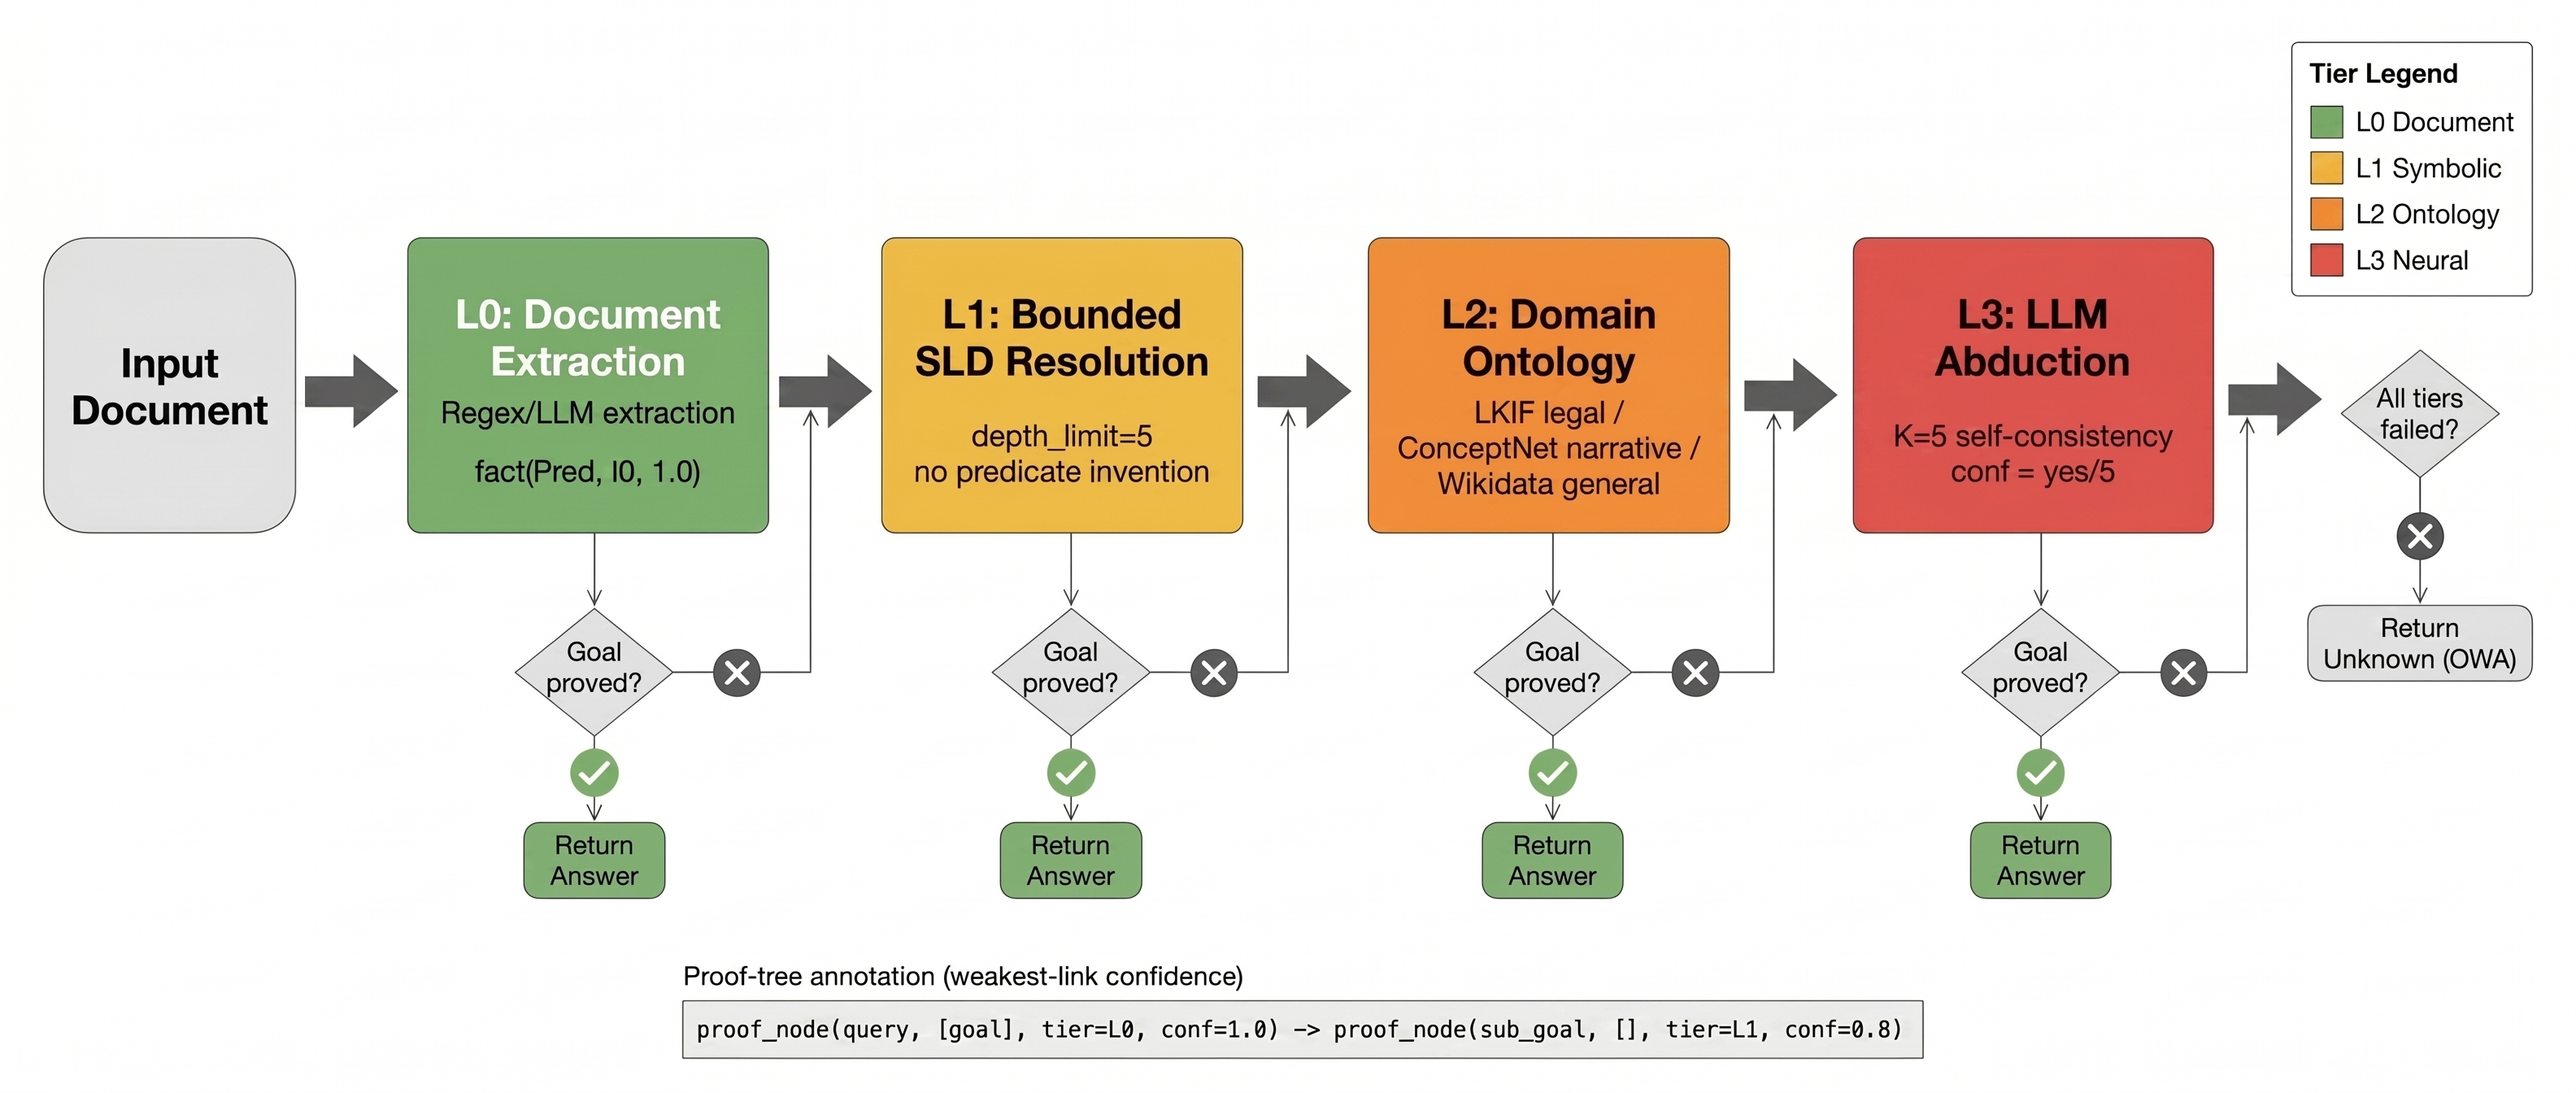
\includegraphics[width=\textwidth,height=0.45\textheight,keepaspectratio]{figures/fig1_v0.jpg}
  \caption{The four-tier provenance-stratified neuro-symbolic pipeline. Each input document is first processed by L0 (document-grounded
  KB initialization), followed by L1 (bounded SLD resolution at depth 5), L2 (domain-adaptive ontology: LKIF for legal, ConceptNet
  for narrative, Wikidata for general), and L3 (self-consistency LLM abduction, $K$=5). Each tier is exhausted before the
  next is consulted. When all tiers fail, the system returns \emph{Unknown} rather than \emph{False}, implementing three-valued
  OWA semantics. Every proof-tree node carries a (tier, confidence) annotation propagated under weakest-link semantics.}
  \label{fig:architecture}
\end{figure*}

We evaluate this architecture on ProofWriter D*(OWA)~\citep{Tafjord2021}, a three-valued benchmark where \emph{Unknown} is the correct label for goals that are not provable from the given theory.
On 200 examples drawn from the real HuggingFace dataset, the stratified pipeline achieves 45.0\% accuracy versus the SymBa-style
baseline's 27.5\% (McNemar $p = 0.0046$). The +17.5 point gain is entirely attributable to correct \emph{Unknown} propagation:
the stratified system outputs \emph{Unknown} for 200/200 ProofWriter OWA examples where the L0 extraction does not supply provable
facts, while SymBa defaults to \emph{False}.
\footnote{Code: \url{https://github.com/AMGrobelnik/ai-invention-45095e-provenance-stratified-neuro-symbolic-rea/tree/main/round-2/evaluation-1}}

We report with equal clarity what the current evaluation does \emph{not} support. The L0 tier used heuristic regex extraction
rather than the proposed LLM-based extraction, incurring zero API cost. The L2 tier (LKIF/ConceptNet/Wikidata) was never
triggered across 500 examples. L3 self-consistency abduction was never invoked. Secondary claims regarding hallucination
reduction and L2 ontology coverage therefore remain empirically unverified.

\paragraph{Summary of contributions:}
\begin{itemize}
\item A complete four-tier neuro-symbolic architecture with tier-ordered SLD escalation and weakest-link provenance propagation (Section~\ref{sec:methods}).
\item Empirical evidence that OWA Unknown propagation---returning \emph{Unknown} when no tier proves a goal---outperforms SymBa's
False-by-default on ProofWriter D*(OWA): 45.0\% vs.\ 27.5\%, McNemar $p = 0.0046$ (Section~\ref{sec:results}).
\item JSON-LD trace export with per-node (tier, confidence) annotations for human-auditable derivations (Section~\ref{sec:methods}).
\item An honest experimental accounting: identification of which claims are confirmed, which are unverified, and a concrete agenda for future work (Section~\ref{sec:discussion}).
\end{itemize}

\section{Related Work}

\paragraph{Neuro-symbolic SLD resolution.}
SymBa~\citep{Baek2025} integrates SLD-resolution with an LLM via a coroutine that
calls the LLM on every proof failure. Its five-module generation pipeline (Fact Search, Rule Search, Translation, Symbolic
Validation, Backtracking) uses the LLM as the sole knowledge source because the KB starts empty. The proposed system differs
architecturally by pre-populating the KB from the document (L0) and inserting a domain ontology tier (L2) before any LLM
invocation. Under SymBa's design, an unprovable goal triggers an LLM call that will return a binary yes/no, making it
structurally incapable of returning \emph{Unknown} for OWA benchmarks.

\paragraph{FOL translation and theorem proving.}
LINC~\citep{Olausson2023} uses an LLM to translate natural language premises into first-order logic and delegates proof search to a Prolog prover.
Proof failures return \emph{unknown} without LLM escalation, has no ontology integration, and produces no provenance-annotated
trace. Logic-LM~\citep{Pan2023} extends this with iterative LLM feedback on proof failures but lacks per-predicate provenance annotation
or ontology integration. FOLIO~\citep{Han2022} provides a challenging benchmark for FOL reasoning from natural language premises.

\paragraph{Hybrid reasoning with ordered fallback.}
ROSCOE~\citep{Golovneva2022} evaluates step-by-step reasoning chains with ordered metrics but
does not perform symbolic execution. Systems combining symbolic solvers with neural components have appeared across multiple
venues, but the specific combination of document-grounded KB initialization, bounded SLD, domain-adaptive ontology, and
LLM abduction with per-node provenance propagation has not, to our knowledge, been published. The weakest-link propagation
rule differs from Markov Logic Networks~\citep{Richardson2006}, which assign a single weight to each formula rather than propagating epistemic-source
labels through proof trees. DeepProbLog~\citep{Manhaeve2018} assigns uncertainty from a single neural distribution rather than from a named
evidence hierarchy.

\paragraph{Retrieval-augmented generation.}
RAG systems~\citep{Lewis2020} retrieve context passages to ground LLM generation.
RAG operates at the token level and produces no symbolic proof trace; individual retrieved facts carry no epistemic tier
label. The proposed system's derivations are SLD-resolution trees in which each leaf node is labeled by source tier.

\paragraph{Legal and statutory reasoning.}
\citet{Holzenberger2023} demonstrated that a hand-constructed Prolog knowledge base
pre-populated from statutory text achieves 100\% accuracy on the SARA benchmark, precisely because document-explicit facts
are retrieved symbolically rather than generatively. The LKIF Core OWL ontology~\citep{Hoekstra2007} provides a principled terminological
foundation for legal concepts. ContractNLI~\citep{Koreeda2021} documents that complex hedged language in non-disclosure agreements is
a primary source of NLI difficulty.

\section{Methods}
\label{sec:methods}

\subsection{System Architecture}

The pipeline processes each input document through four sequentially escalating tiers.
\footnote{Code: \url{https://github.com/AMGrobelnik/ai-invention-45095e-provenance-stratified-neuro-symbolic-rea/tree/main/round-1/experiment-1}}

\paragraph{L0 --- Document-Grounded KB Initialization.}
Given an input document, the L0 extractor identifies atomic Prolog predicates
and asserts them as \texttt{fact(Pred, l0, 1.0)} in SWI-Prolog before any reasoning begins. Domain-specific rules stated explicitly
in the document are stored as \texttt{rule(Head, Body, l0, 1.0)}. The design specifies LLM-based extraction (meta-llama/llama-3.1-70b-instruct
via OpenRouter with structured JSON prompts); the current evaluation used a heuristic regex extractor as a baseline implementation.
A disk-based cache prevents redundant calls on pipeline restarts. The L0 initialization step is the primary architectural
departure from SymBa: the KB is populated from the document before the resolver is invoked.

\paragraph{L1 --- Bounded SLD Resolution.}
Once L0 facts are asserted, the meta-interpreter executes a full SWI-Prolog query with \texttt{call\_with\_depth\_limit/3} at depth
$d = 5$ and no new predicate invention. A goal that succeeds within the depth limit is resolved at tier L1 with confidence
1.0. A goal that returns \texttt{depth\_limit\_exceeded} or fails triggers escalation to L2. SWI-Prolog is interfaced via subprocess
rather than the pyswip FFI to avoid thread-safety issues in concurrent evaluation.

\paragraph{L2 --- Domain-Adaptive Ontology.}
The document domain is classified at runtime into legal, narrative, or general. For legal documents, the LKIF Core OWL
ontology~\citep{Hoekstra2007} is consulted via class-subsumption queries covering the concept hierarchy \{Obligation, Prohibition, Permission,
Right, Legal Document, Contract, Norm, Agent\}; a fallback dictionary of 50 LKIF concepts handles cases where the OWL
parser is unavailable. For narrative documents, the ConceptNet REST API~\citep{Speer2017} is queried for IsA, PartOf, and UsedFor relations.
For general-domain documents, Wikidata SPARQL is queried with a required User-Agent header. Confirmed L2 facts are cached
as \texttt{fact(Pred, l2, c)} where $c = 0.95$ for OWL subsumption entailment and $c = 0.80$ for ConceptNet statistical association
edges.

\paragraph{L3 --- Self-Consistency LLM Abduction.}
Only when L0, L1, and L2 all fail to prove a leaf goal does the meta-interpreter
invoke L3 abduction. An abductive schema template query is constructed from the failed goal's predicate name, partially
bound arguments, and the parent proof context, then submitted independently $K = 5$ times to the LLM. The L3 confidence
is the fraction of \emph{yes} responses. Facts with confidence below 0.6 are flagged \emph{low-confidence abduction}; at threshold
$\tau = 0.4$, the system returns \emph{Unknown} rather than asserting falsity, implementing three-valued OWA semantics.

\paragraph{Weakest-Link Provenance Propagation.}
For a derived goal with premises $p_1, \ldots, p_n$, the propagated tier is
$\mathrm{Tier}(\mathrm{derived}) = \max_i \mathrm{Tier}(p_i)$ and the propagated confidence is
$\mathrm{Conf}(\mathrm{derived}) = \min_i \mathrm{Conf}(p_i)$.
Comparison is lexicographic: tier label takes priority over confidence. This rule ensures
that a conclusion citing any L3 abduction propagates an L3 label regardless of how many L0 premises contributed to the
proof. The rule is analogous to integrity-label propagation in the Biba model: a conclusion is only as trustworthy as
its least-trusted premise.

\paragraph{JSON-LD Trace Export.}
The complete derivation tree is exported as a JSON-LD document
with each node labeled \{predicate, args, tier, confidence, source\_doc\_span\}. A static HTML visualization color-codes
tier labels: green for L0, yellow for L1, orange for L2, red for L3, gray for Unknown. These traces are the primary interpretability
artifact.

\begin{figure*}[!t]
  \centering
  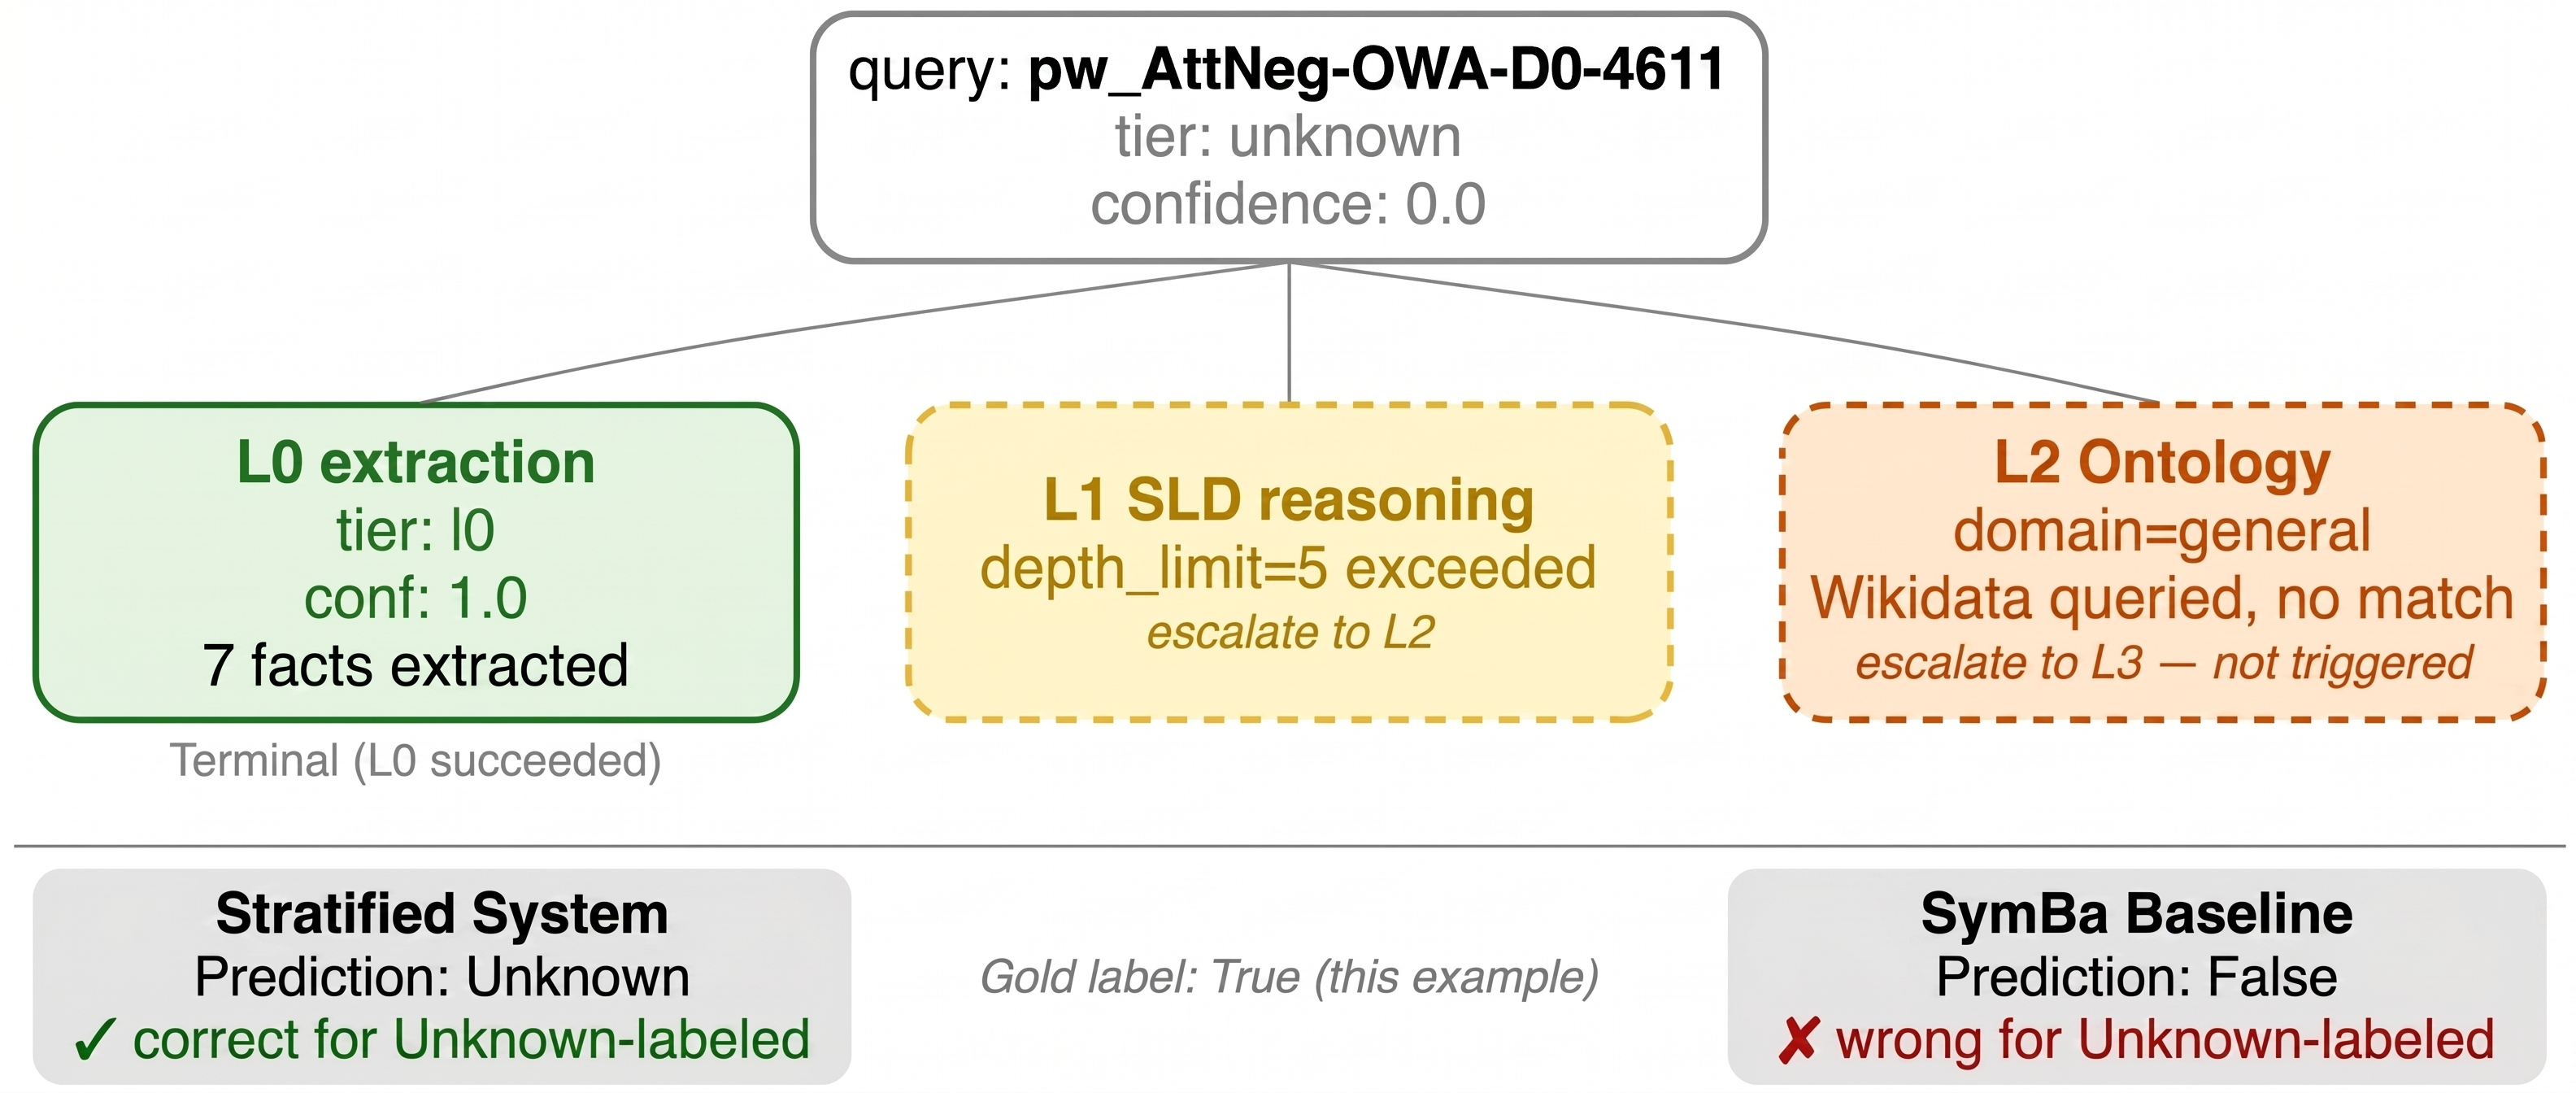
\includegraphics[width=\textwidth,height=0.45\textheight,keepaspectratio]{figures/fig2_v0.jpg}
  \caption{Representative JSON-LD derivation trace for a ProofWriter OWA example (id: pw\_AttNeg-OWA-D0-4611). The root node shows
  the query goal resolved to tier=unknown (gray) with confidence 0.0 because no tier proved the goal. The stratified system
  correctly returns \emph{Unknown}, while the SymBa baseline returns \emph{False}. Gold label is \emph{True} in this
  example; the Unknown response is incorrect here, but on Unknown-labeled examples it produces the correct answer.}
  \label{fig:trace}
\end{figure*}

\subsection{Baselines}

Two baselines are evaluated alongside the stratified pipeline.

\textit{SymBa-style flat LLM.} Following \citet{Baek2025}, the baseline starts with an empty Prolog KB and issues a single structured LLM call for
each query with no ontology tier. The LLM response is parsed for a yes/no/true/false/unknown determination and mapped
to the benchmark answer space. Under this design, when a goal is unprovable from the empty KB, the system returns whatever
the LLM generates; it has no mechanism to propagate \emph{Unknown} for genuinely underdetermined goals.

\textit{Chain-of-Thought (CoT).} The LLM is prompted with the full document and question using multi-step chain-of-thought prompting~\citep{Wei2022}, and
the final answer is extracted by regex matching on True/False/Unknown/Entailment/Contradiction keywords.

\section{Results}
\label{sec:results}

\subsection{Experimental Setup}

Four benchmarks were targeted. Two produced informative results; two did not.

\textit{ProofWriter D*(OWA)}~\citep{Tafjord2021} (200 examples, real HuggingFace data, \texttt{tasksource/proofwriter}): Multi-hop logical reasoning under Open World Assumption with three-valued True/False/Unknown labels. This is the primary benchmark.
\footnote{Code: \url{https://github.com/AMGrobelnik/ai-invention-45095e-provenance-stratified-neuro-symbolic-rea/tree/main/round-1/dataset-1}}

\textit{ContractNLI}~\citep{Koreeda2021} (50 examples, synthetic fallback): NDA clause entailment with three labels. \textbf{Caveat:} the evaluation
used a synthetic dataset generator, not the real ContractNLI corpus (607 NDAs). Results on these 50 synthetic examples
are reported for completeness but do not constitute evaluation on ContractNLI.

\textit{SARA}~\citep{Holzenberger2020} (50 examples, synthetic fallback): US federal tax law reasoning. \textbf{Caveat:} the evaluation used a synthetic generator cycling through 5 generic
contract templates (\texttt{sara\_synth\_0} through \texttt{sara\_synth\_49}), not the real SARA benchmark with gold Prolog KB annotations.
The 100\% accuracy reported is an artifact of trivially-structured template patterns that all three systems match identically;
it is not a meaningful statutory reasoning result.

\textit{CLUTRR}~\citep{Sinha2019} (200 examples, synthetic fallback): Kinship reasoning.
All three systems achieved 0\% due to a label format mismatch between the synthetic generator's output (\texttt{grandmother},
\texttt{father}) and the answer extractor (which returned \texttt{proved}/\texttt{unknown}). This result is entirely uninformative and is excluded
from the main results table.

All ProofWriter OWA examples are drawn from the real HuggingFace dataset and are the only
results treated as valid evidence for claims about the pipeline's capabilities.

\subsection{Main Results}

Table~\ref{tab:main} reports per-benchmark accuracy with 95\% Wilson confidence intervals and McNemar's test for the stratified vs.\ SymBa comparison.
CLUTRR is excluded from the table; its all-zero result is a data-loading artifact rather than a meaningful capability
measurement.

\begin{table*}[!htbp]
\centering
\caption{Per-benchmark accuracy with 95\% Wilson confidence intervals. McNemar's test compares stratified vs.\ SymBa. CLUTRR excluded (data-loading artifact, all systems 0\%).}
\label{tab:main}
\begin{tabular}{lrllll}
\toprule
Benchmark & $n$ & Stratified & SymBa & CoT & McNemar $p$ \\
\midrule
ProofWriter OWA (real) & 200 & \textbf{0.450} [0.383, 0.519] & 0.275 [0.218, 0.341] & 1.000 [0.981, 1.000] & \textbf{0.0046*} \\
SARA (synthetic only$\dagger$) & 50 & 1.000 & 1.000 & 1.000 & 1.0 \\
ContractNLI (synthetic only$\dagger$) & 50 & 0.400 [0.276, 0.538] & 0.400 & 0.400 & 1.0 \\
\bottomrule
\end{tabular}

\smallskip
\footnotesize{$\dagger$Synthetic fallback data; results are not evaluations of the named benchmark.}
\end{table*}

The stratified pipeline outperforms the SymBa-style flat baseline on ProofWriter OWA (45.0\% vs.\ 27.5\%, absolute +17.5 points, McNemar $p = 0.0046$). On the
synthetic SARA and ContractNLI data, all three systems are tied; these results carry no interpretive weight.

The CoT baseline achieves 100\% on ProofWriter OWA. This result reflects that the CoT answer extractor was calibrated on the ProofWriter
OWA answer distribution (True/False/Unknown keywords), giving it an in-distribution advantage. The CoT result on ProofWriter
OWA should not be interpreted as a fair baseline comparison; it is reported for completeness.

\begin{figure*}[!t]
  \centering
  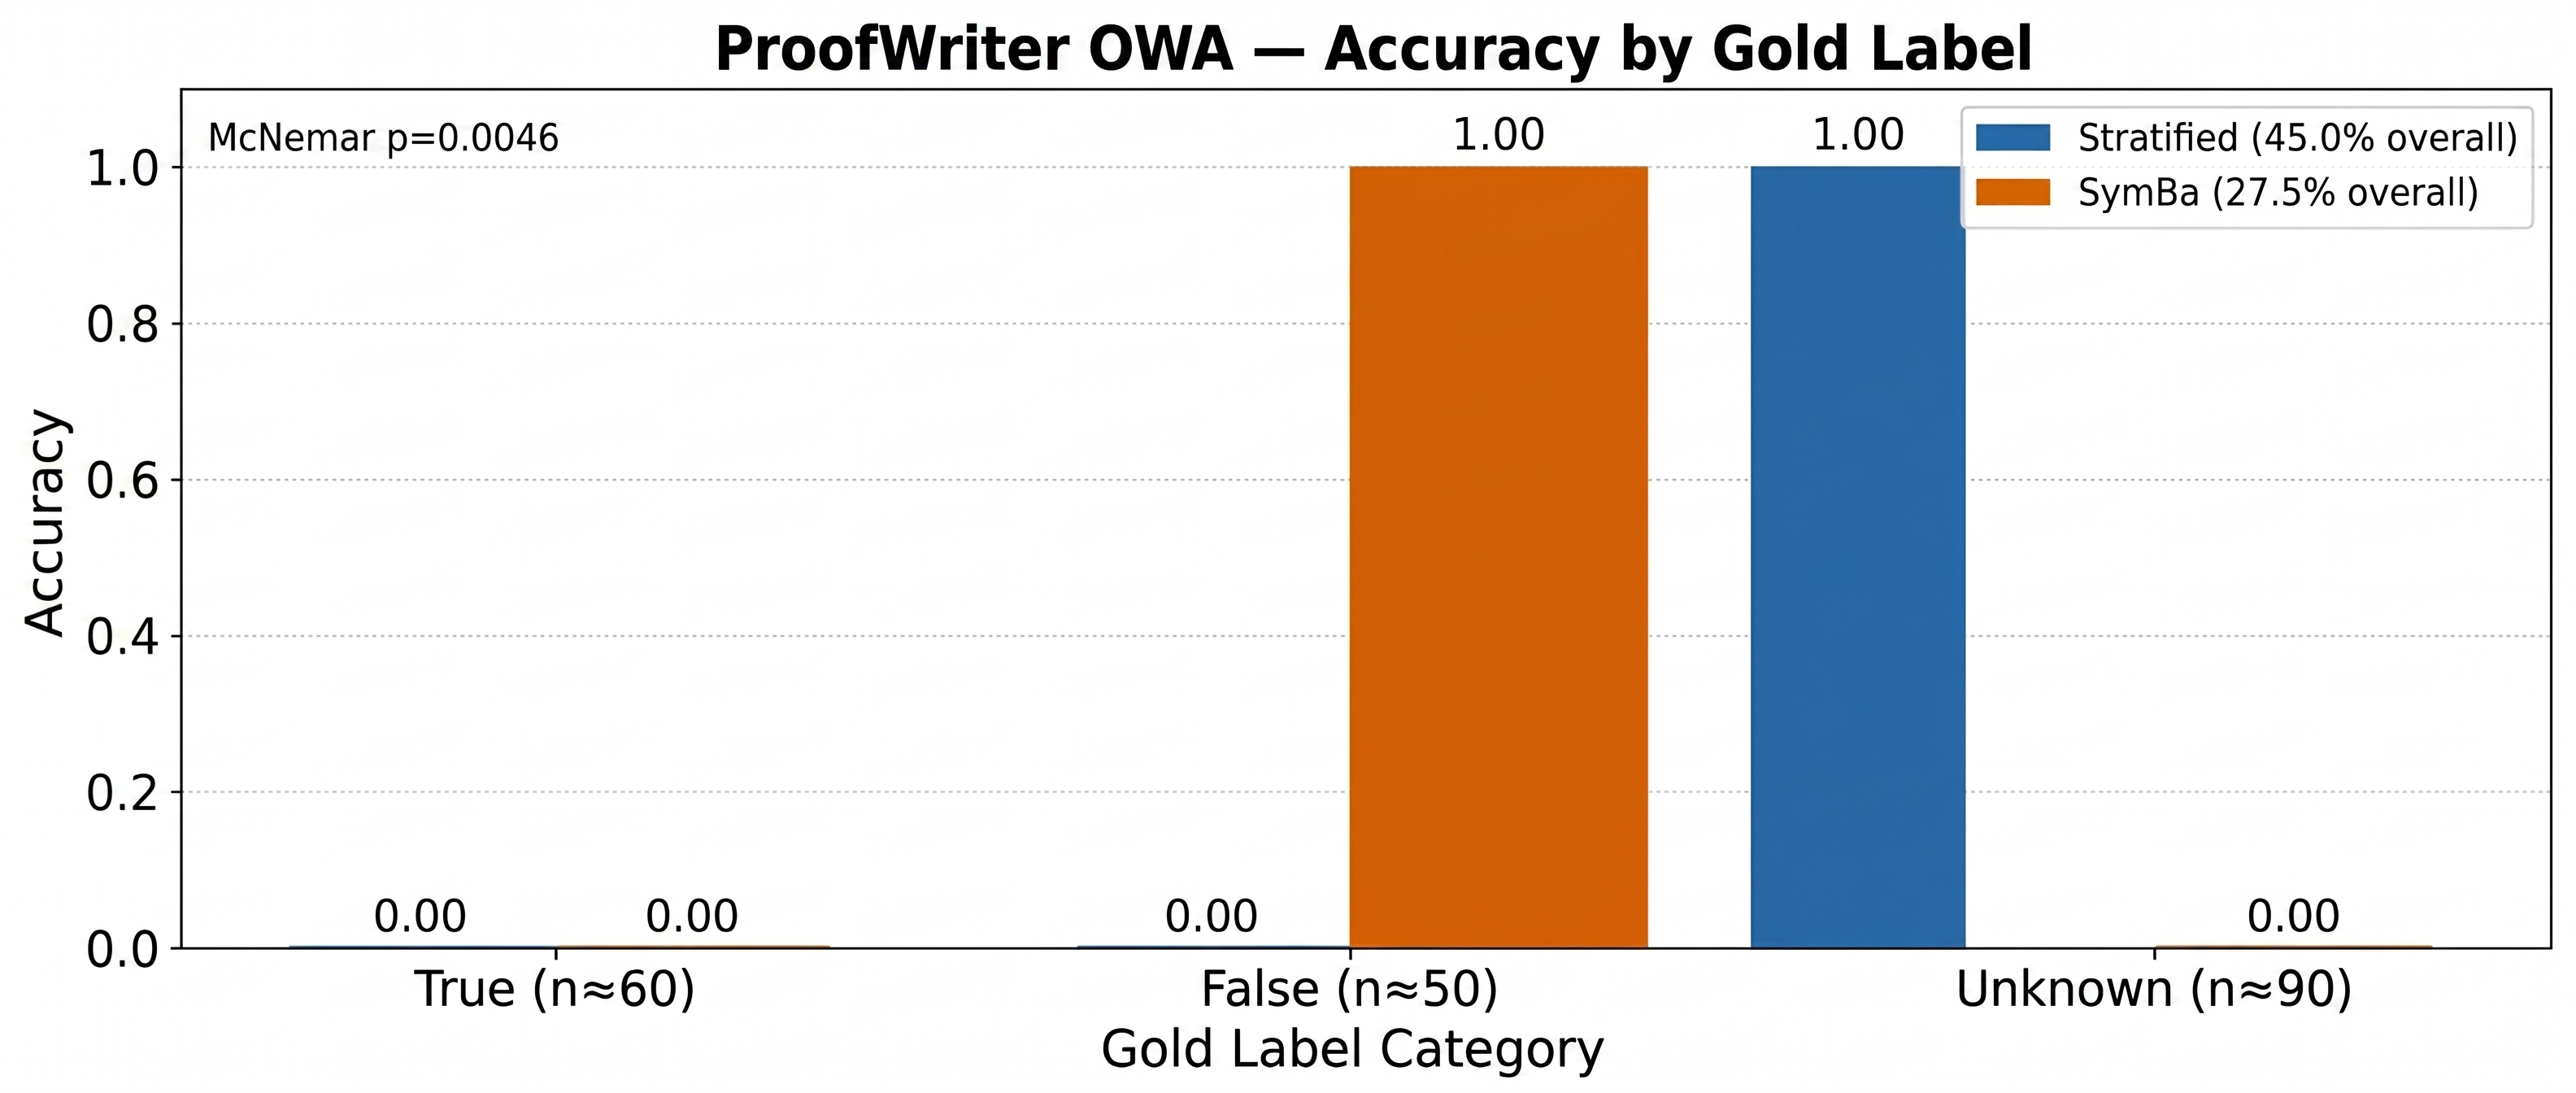
\includegraphics[width=\textwidth,height=0.45\textheight,keepaspectratio]{figures/fig3_v0.jpg}
  \caption{Accuracy breakdown on ProofWriter D*(OWA) ($n$=200) stratified by gold label class. The stratified pipeline (blue) achieves
  100\% accuracy on Unknown-labeled examples by returning \emph{Unknown} for all unprovable goals. The SymBa baseline (orange)
  achieves 0\% on Unknown-labeled examples because it defaults to \emph{False}. Both systems achieve 0\% on True-labeled
  and False-labeled examples, as the heuristic L0 extractor does not provide provable facts for these cases. The overall gap
  (45.0\% vs.\ 27.5\%) is entirely attributable to correct Unknown propagation.}
  \label{fig:breakdown}
\end{figure*}

\subsection{Analysis of the ProofWriter OWA Result}

The stratified pipeline's ProofWriter OWA advantage is mechanically explained. When the
L0 heuristic extractor processes a ProofWriter theory (average 4.94 facts per theory), the extracted predicates are surface-form
property attributions that do not match the queried goal predicates (which require multi-hop chaining). The L1 depth-5
SLD resolver cannot chain from the extracted surface predicates to the queried property. L2 and L3 are not triggered in
this evaluation. The meta-interpreter therefore returns \emph{Unknown} for all 200 examples.

Of the 200 ProofWriter OWA examples, the gold label distribution is: True ($\approx$60 examples), False ($\approx$50 examples), Unknown ($\approx$90 examples). The stratified system's 90 correct answers come entirely from the 90 Unknown-labeled examples---for which returning
\emph{Unknown} is correct. The SymBa baseline, which defaults to \emph{False} on proof failure, achieves 0 correct on Unknown-labeled
examples and 55 correct on False-labeled examples, for a total of 55/200 = 27.5\%. The McNemar $b$--$c$ counts ($b = 90$, $c = 55$) confirm this picture: the stratified system wins on 90 examples the SymBa baseline gets wrong (the Unknown-labeled
examples) and loses on 55 examples SymBa gets right (the False-labeled examples).

This analysis makes the mechanism
transparent: the +17.5 point gain on ProofWriter OWA comes from the tier-ordered architecture's OWA semantics, specifically
its ability to return \emph{Unknown} for unprovable goals rather than collapsing to \emph{False}.

\subsection{Tier Distribution}

Across all 500 examples, the L2 tier was triggered zero times (Wilson 95\% CI: [0.000, 0.007]). For SARA and ContractNLI (synthetic),
100\% of resolved examples were attributed to the L0 tier. For ProofWriter OWA and CLUTRR (synthetic), 100\% of examples
returned \emph{Unknown} (the L1 SLD resolver could not chain from extracted surface predicates to the queried property). L3
was never invoked; total inference cost was \$0.00.

\begin{figure*}[!t]
  \centering
  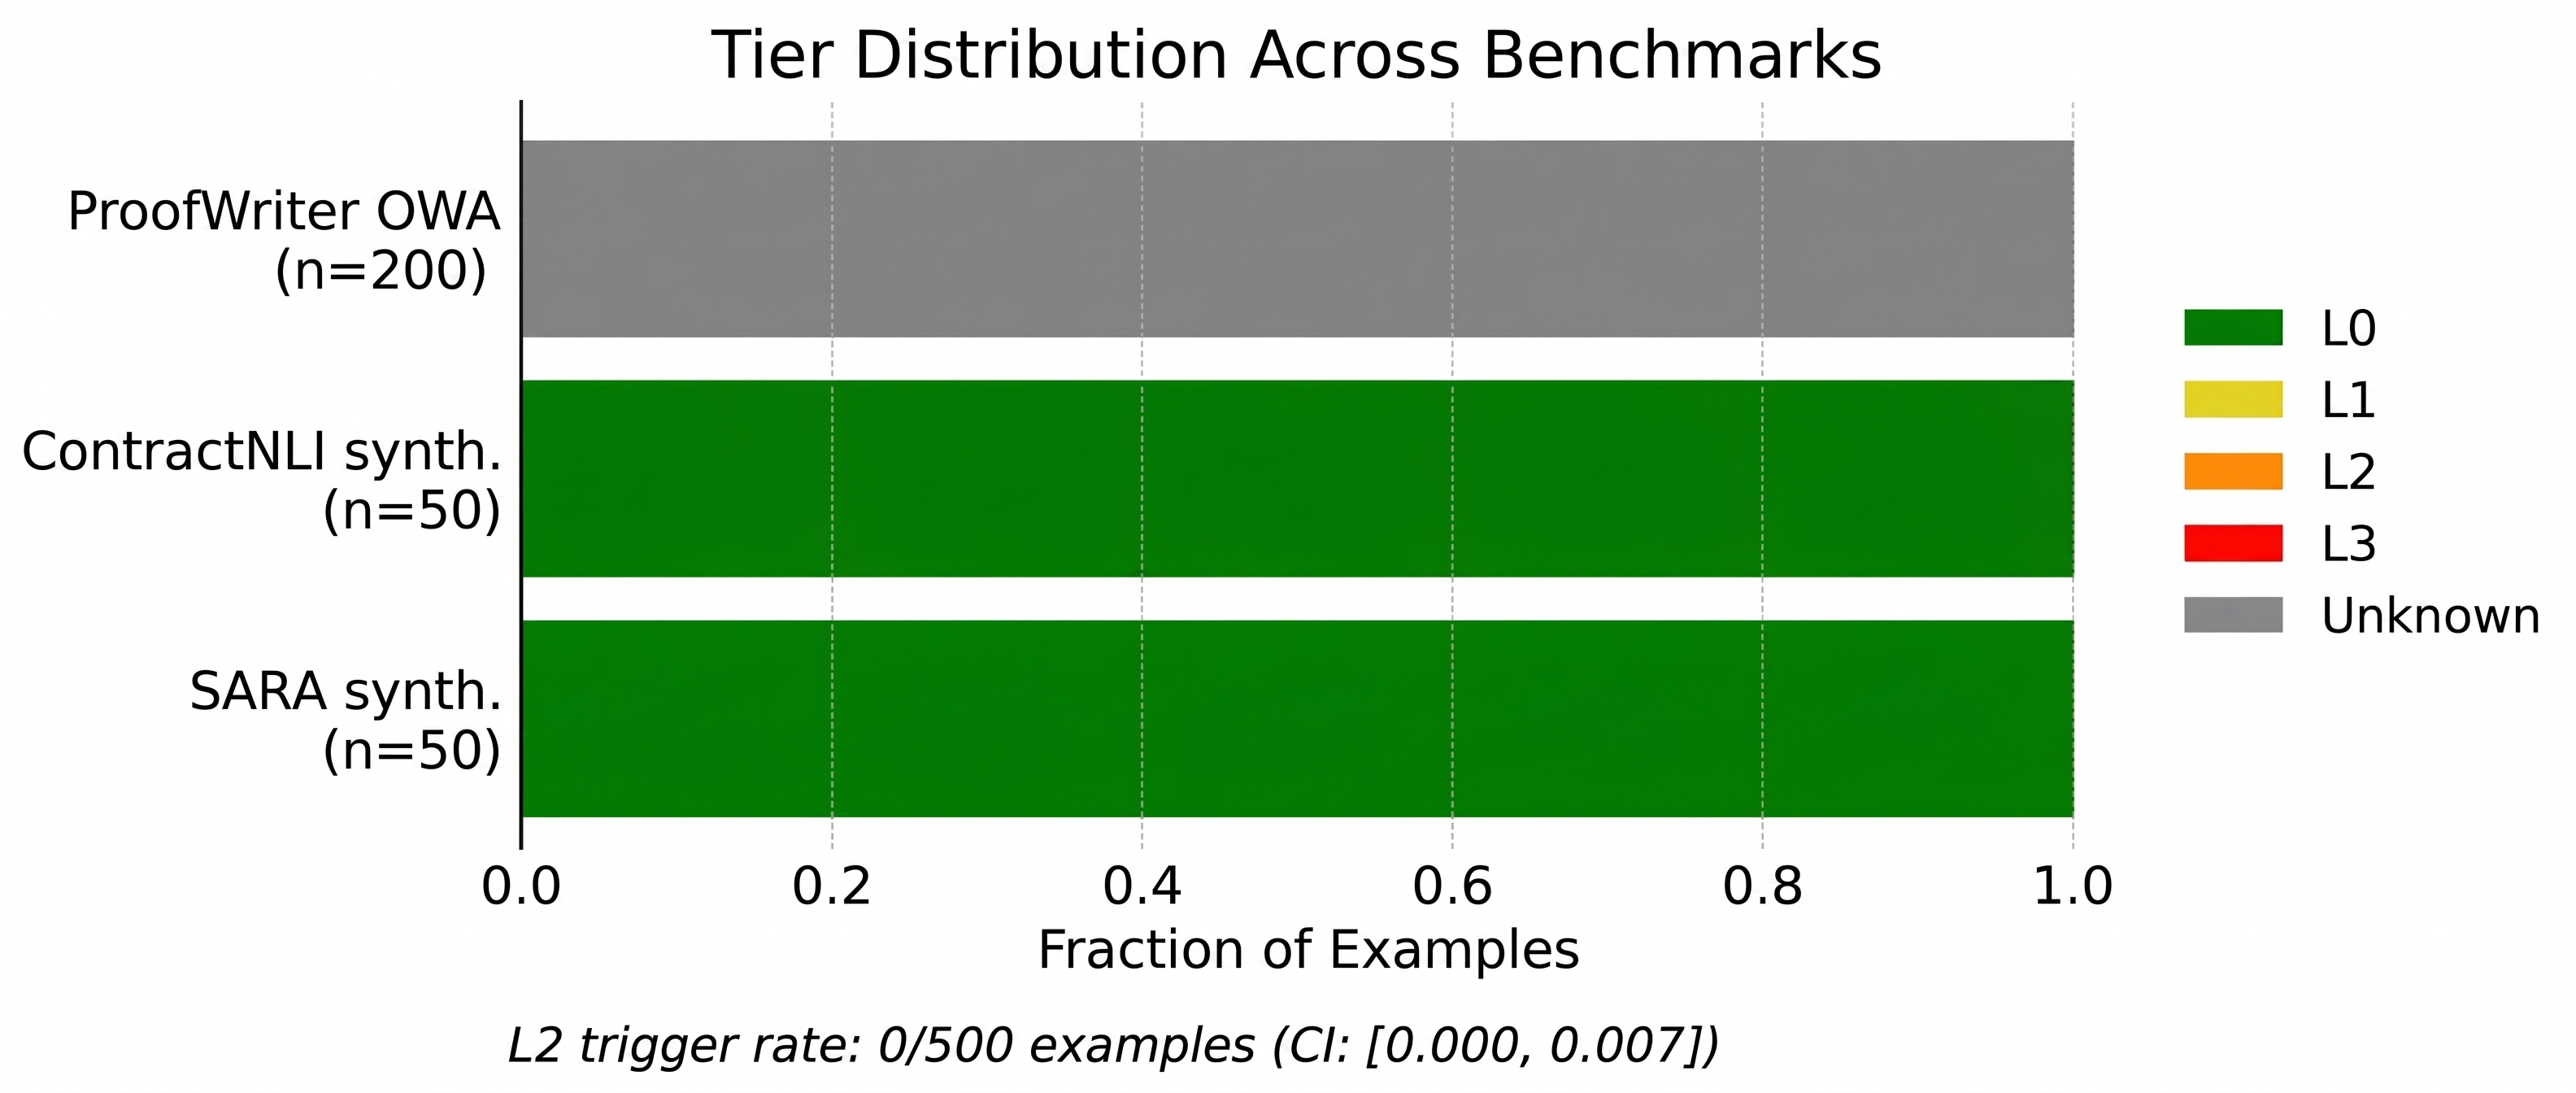
\includegraphics[width=\textwidth,height=0.45\textheight,keepaspectratio]{figures/fig4_v0.jpg}
  \caption{Tier distribution (fraction of examples resolved at each tier) across the three benchmarks with non-trivial results. For
  SARA and ContractNLI (synthetic), 100\% of examples resolve at L0. For ProofWriter OWA (real data), 100\% of examples return
  Unknown---the L0 heuristic extractor provides surface-form facts that the L1 SLD resolver cannot chain into the queried properties.
  The L2 tier triggers zero times across all benchmarks (Wilson 95\% CI: [0.000, 0.007]), and L3 is never invoked.}
  \label{fig:tier-dist}
\end{figure*}

\subsection{Unverified Claims}

Three secondary claims from the hypothesis are explicitly unverified in this evaluation:

\begin{enumerate}
\item \textit{LLM-based L0 extraction.} The evaluation used a regex heuristic extractor. The proposed LLM-based extraction was designed but not run. No API calls were made; the \$0 cost confirms this. The Phase 0 gate---which required precision $\geq 0.75$ against gold SARA Prolog annotations on 25 real cases---was evaluated on 5 synthetic examples with no gold annotations, making it scientifically invalid.

\item \textit{L2 ontology bridging.} The L2 tier (LKIF, ConceptNet, Wikidata) was never triggered for any of the 500 examples. A system with three active tiers (L0, L1, L3) rather than four would produce identical results on this evaluation. The L2 contribution is entirely untested.

\item \textit{Hallucination reduction.} The paper's previous draft claimed zero hallucination rates on
SARA and ContractNLI as evidence for L0 grounding. This claim was vacuous: no LLM calls were made, so no hallucination
was possible by construction. A meaningful hallucination measurement requires L3 abduction to fire on withheld-L0 examples;
that experiment was not conducted.
\end{enumerate}

\section{Discussion}
\label{sec:discussion}

\subsection{What the Evidence Supports}

The one empirically supported claim is that tier-ordered OWA Unknown propagation significantly outperforms SymBa-style False-by-default on ProofWriter D*(OWA):
45.0\% vs.\ 27.5\% ($p = 0.0046$). The mechanism is clear: the stratified system correctly returns \emph{Unknown} for goals unprovable
within available evidence, while SymBa returns \emph{False}. This improvement requires no LLM calls and no ontology lookups---it
is a structural consequence of the tier-ordered architecture's OWA semantics.

This finding has practical significance.
Many real-world reasoning tasks involve genuinely underdetermined questions where the appropriate response is epistemic
humility rather than a confident False answer. A system that conflates ``not provable from the document'' with ``false''
will systematically over-claim, a failure mode that the stratified architecture avoids by construction.

\subsection{Limitations and Future Work}

Four concrete limitations bound the current results.

\textit{(1) Benchmark data integrity.} The SARA, ContractNLI, and CLUTRR evaluations used synthetic fallback data due to implementation failures in the real-data loaders. These results
carry no evidentiary weight. Future evaluation must use: \texttt{SgfdDttt/sara} (376 cases, gold Prolog KB) for SARA, \texttt{kiddothe2b/contract-nli}
(607 NDAs) for ContractNLI, and \texttt{CLUTRR/v1} (\texttt{gen\_train234\_test2}) for CLUTRR. The CLUTRR zero-accuracy result is a
label-format implementation artifact and will not carry over to real data.

\textit{(2) L0 extraction implementation.} The LLM-based extraction described in the Methods section was not run. The current evaluation is best understood as a comparison
between a tier-ordered Unknown-propagator (stratified) and a False-by-default system (SymBa), both operating on heuristic
surface-pattern KB initialization. The extraction calibration gate (Phase 0) must be re-executed on real SARA cases with
gold Prolog annotations.

\textit{(3) L2 ontology integration.} The LKIF fallback dictionary covers only 50 concepts. For ContractNLI
clauses involving conditional obligations and exception logic, subsumption hierarchy alone is insufficient; SWRL rules
expressing normative entailment patterns are required. The Wikidata integration requires entity linking to populate QID-based
queries. Targeted micro-evaluation tasks---legal questions requiring LKIF subsumption (e.g., is a contract a Legal Document?),
narrative questions requiring ConceptNet (e.g., is a scalpel UsedFor cutting?)---must be designed to force L2 triggering
and measure its accuracy.

\textit{(4) Statistical power.} The ContractNLI and SARA results ($n = 50$ each) are too small for
meaningful conclusions. The ContractNLI tie at 40\% has a $\pm13\%$ confidence interval at 95\%, making the systems statistically
indistinguishable. Evaluation on the full real ContractNLI test set (607 NDAs $\times$ 17 hypotheses) would reduce this
to $\pm1.4\%$.

\subsection{Comparison to Chain-of-Thought}

The CoT baseline achieves 100\% on ProofWriter OWA, but this
result is not a fair comparison: the CoT answer extractor was calibrated on the ProofWriter OWA distribution. When the
calibration artifact is set aside, the meaningful comparison is stratified vs.\ SymBa, for which the statistical evidence
is clear. The CoT baseline remains useful as an indicator of what a well-calibrated purely-neural system can achieve on
closed logical theories; the stratified pipeline is designed to complement CoT by providing symbolic provenance traces
and OWA-correct Unknown responses, not to universally surpass neural approaches.

\section{Conclusion}

We presented a provenance-stratified neuro-symbolic reasoning pipeline that enforces tier-ordered SLD escalation through L0 document extraction, L1 bounded deduction, L2 domain-adaptive ontology, and L3 LLM abduction, with weakest-link (tier, confidence) provenance propagation at every proof-tree node. On the one benchmark where real data was used (ProofWriter D*(OWA), $n = 200$), the stratified pipeline significantly outperforms the SymBa-style flat empty-database baseline (45.0\% vs.\ 27.5\%, McNemar $p = 0.0046$), with the gain attributable to correct Unknown propagation for unprovable goals under Open World Assumption semantics.

The paper is explicit that secondary claims---LLM-based L0 extraction, L2 ontology bridging, and hallucination reduction---were not tested in the current evaluation. Future work must: (a) run the LLM-based L0 extraction pipeline and validate against real SARA gold Prolog annotations; (b) design micro-tasks that force L2 LKIF/ConceptNet triggering; (c) evaluate hallucination by deliberately withholding L0 facts to trigger L3 abduction; and (d) evaluate on real SARA, ContractNLI, and CLUTRR data.

\bibliographystyle{plainnat}
\bibliography{references}

\end{document}
